

\subsubsection{KW48: 29.11.2021 bis 05.12.2021}
\begin{quote}
	\begin{figure}
		\centering
		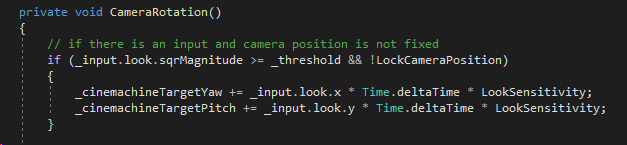
\includegraphics[width=0.7\linewidth]{img/SemihSoenmez_IMG/screenshot001}
		\caption{}
		\label{CodeKamera}
	\end{figure}
	
	\subsubsection*{Arbeit in der Schule}
	Antrag für Unity-Spielumgebung an Herrn Rusch geschrieben.

	\subsubsection*{Arbeit außerhalb der Schule}
	- Die Umgebung gekauft und heruntergeladen
	
	- Im packet-manager, die Umgebung in das Projekt importiert
	
	- SchoolScene geöffnet
	
	- Meine Charaktere in die Umgebung eingefügt, die jedoch nicht funktioniert haben
	
	- Ein funktionierendes Charakter gefunden und eingefügt
	
	- Charakter mit Cinemachine verbunden: Kamera folgt dem Charakter
	
	- Die Kamera, die man mit der Maus bewegen kann ist zu schnell, deshalb wurde im Code folgende Änderungen vorgenommen um die Sensivität einzustellen. Abbildung\ref{CodeKamera}
	Eine neue Variable LookSensivity wurde definiert und mit der x y Werte von der Kamera multipliziert. Da die Variable public definiert wurde kann sie jeder Zeit im Inspektor Menü verändert werden.
	
	-
	
		
	
	\subsubsection*{Welche Schwierigkeiten hat es gegeben}
	
\end{quote}

